\section[Data hybridization]{Aim 2 - Data hybridization for population mapping in Niger}

Our third and final project pertains to the combination of data sources from outside the health systems to produce relevant information on populations in developing countries. If the low quality or even the lack of existence of good data on populations size and locations is well known in low resource and developing countries, there is a high quantity of data source, sometimes openly accessible, that can help documenting where people live, and who they are.

This  project is exploring an innovative approach to mapping of populations in resource-limited settings. Using voters registration lists, to our knowledge a data source seldom used in demography, we will offer a map of population in Niger that will be callable and usable by different actors intervening in Niger. To do this, we will challenge current practice in population mapping, and will aim at producing a point map, more adapted to daily usage than raster surfaces.

\subsection{Mapping Sahel populations}

In countries that were formerly part of the French colonial empire, investments necessary to produce geolocalized data on population have seldom been done. Paul Pelet's 1902 very first \textit{Atlas des colonies française} did not include a lot of
information outside of topographic data\cite{zimmermann_atlas_1903}. Additionally, there was a radical choice made to use spellings for places in colonies that were adapted to metropolitan French rather than to local languages\cite{zimmermann_atlas_1903}

Meanwhile, In contrast to geological data or natural features, population is non continuous in space, and is changing fast. In 1935, Fawcett discerned three facts one may want to describe in a population map \cite{fawcett_population_1935}:
\begin{enumerate}
	\item The actual number of the people within given areas
	\item The density of the population
	\item The grouping, or arrangement, of the population.
\end{enumerate}

Each of these facts require a different mapping and require different amounts and nature of primary data, and different computational approaches. The latest advances in population mapping are geared towards the production of density surfaces, presenting a continuous description of where populations live on a territory\cite{linard_population_2012}. This new approach is made possible by the availability of large datasets for land use, and other usable covariates and the computational ability to interpolate these  different data sources for population distribution\cite{stevens_disaggregating_2015}.

Meanwhile, this approach presents two main problems that make its result of little use in country like Niger. First, the output format if these maps, a raster of population distribution, is of little use at a local level, where actors typically use place names and not GPS coordinates. Second, in countries with little urbanization, and poor population data, these rasters end up displaying an overlay of covariate layers more than they present a credible distribution of populations. Moreover, if this top-down approach is useful to provide macro-level perspectives on population distribution, it is not useful for local level use. Local actors typically think in terms of places names, more than in terms of GPS coordinates. Additionally, the attractivity of urban centers for rural population is hard to model through macro level covariates, as it often depends on such factors as tradition, habits or administrative border drawing, as is evident in Figure \ref{AfriPopMap}.

\begin{figure}
	\begin{center}
	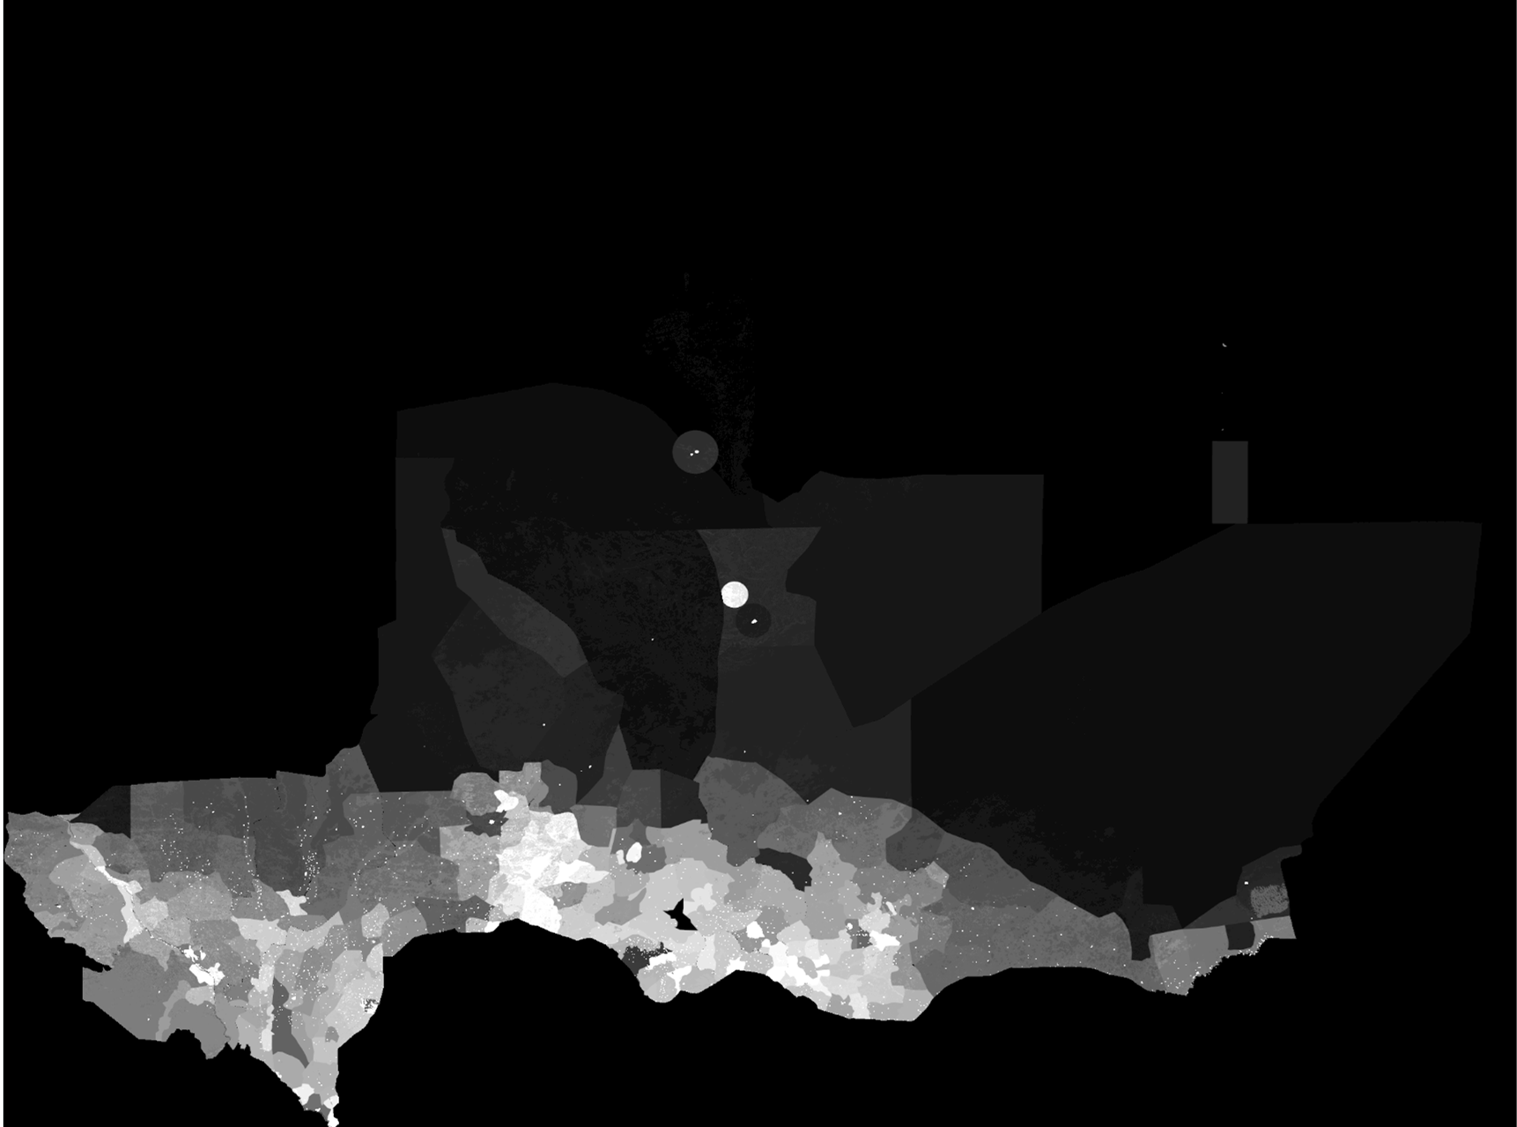
\includegraphics[width=0.8\textwidth]{figure/WORLDPOP_Niger.png}
	\caption{Mapping of Niger population from AFRIPOP}
	\label{AfriPopMap}
	\end{center}
\end{figure}

To offer more useful maps for local actors, I will use an approach supported by minimal modelling of primary population data distribution, and geared towards the anchoring of population in callable localization names.

\subsection{Data}

\paragraph{Voters list as a demographic Datasource} A data source that is, to our knowledge, seldom used to inform population mapping for public health purposes, is voters registration lists. There is meanwhile a case for the use of voters' registration data to estimate size of populations. By definition, voters' registration should aim at being as complete as possible a register of adults in the nation. Moreover, in most democracies, some form of national elections are held at least  every five years, leading to an update at least partial of voters' registrations. In sub-Saharan Africa, between the years 2015 and 2016, 27 countries were supposed to hold national elections, leading to a theoretical registration of more than half of the adult population of the continent. Finally, for transparency and accountability reasons, electors registries are usually supposed to be accessible. \cite{spiegelhalter_handling_2005}

Due to the sensitive and political use of these data, the quality of voters registries are often described as not being trustworthy. On other hand, for the same sensitivity reasons, voters registries are receiving a high level of scrutiny from different actors, and are audited sometimes multiple times before validation. This level of scrutiny before validation is much higher than the attention given to a lot of studies or other often used data sources.

\paragraph{The Niger 2016 elections voters registry} In Niger, presidential and parliamentary elections were held in February 2016. Voters lists were updated during the second half of the year 2015, under the supervision and control of a mission of the Office International de la Francophonie (OIF). The operations for registration of voters were conducted during the third quarter of 2015\footnote{\url{http://www.ceni-niger.org/article-region/##more-24}}.
A first version of the voters list was published on December 21, 2015, tallying 7,569,172 voters, out of 8,569,309 that were expected based on the 2012 census\footnote{\url{http://www.iinanews.org/page/public/news_details.aspx?id=98929&NL=True}}

Final lists were validated in early January 2016 after being corrected for some incoherencies noted by the supervisory body\footnote{\url{http://www.nigerinter.com/2016/01/le-fichier-electoral-du-niger-valable-sous-reserves/}}.
A final report on these lists was published in may 2016\footnote{\url{http://www.nigerinter.com/2016/05/remise-officielle-du-rapport-du-fichier-electoral-au-ministre-detat-a-linterieur-par-le-cfeb/}}.
The Comission Electorale Nationale Independante (CENI) later made these lists fully available on its website, from which I extracted, anonymized and formatted the lists.

\paragraph{RENALOC and RENACOM} The \textit{Répertoire National des Localités} (RENALOC) is a geolocalized repertory of all localities in Niger.  The 2012 version was downloaded as a pdf file from the \textit{Institut National de la Statistique} (INS) website. The tables were extracted in bulk from this file using the Tabula Package, and then processed in Python to recompose the geographic structure of the document. The final data consists in 34507 localities, for which the INS provides the number of inhabitants, by gender, as well as the number of households, and the number of agricultural households. For most of the localities, a GPS coordinate is recorded, as well as the type of locality (neighborhood, village, camp, water well, hamlet).

The 2006 version, named RENACOM, was retrieved in tabular format directly from the INS website.

\paragraph{OpenStreetMap} Additional geolocalization method will be extracted from OpenStreetMap (OSM), using the python API for OSM.

\subsection{Methods}

This project has three main components.

\subsubsection{Name Matching}

Due to the history of the creation and administration of the Nigerien territory, different spellings are in use for most localities in Niger. There are no obvious reasons to prioritize one spelling over another for this project. To the contrary, I want users to be able to use whichever spelling of a name they prefer to query their results.

In collaboration with a student in the department of Computer Science, I am designing a matching algorithm for different spellings of the same locality names in Niger. Our approach relies on the use of  a mixture of standard string matching algorithms. We use these algorithms for each pair of data sources and define a heuristic to combine them and select best matches. We also enrich these heuristics by defining patterns and features that allow a first classification and simplification of names to improve matching performance. These patterns may be data source specific to reflect specific explicit or non-explicit conventions used in each data source.

After this first round of unsupervised matching, we will manually confirm some of the matches with the help of members of the OSM community in Niger. Using this validated training set, we will fit supervised algorithms to improve our previous matching approach.

As a result of this step, I will have a consolidated list of localities in Niger, with different possible spellings of names for each of them.

\subsubsection{Locality mapping}

The three data sources that include GPS coordinates (RENALOC, RENACOM, OSM) have GPS coordinates for different subsets of localities in Niger. It appears that RENALOC GPS coordinates are biased, and that OSM coordinates are sometimes rough estimates of exact locations with a rounding factor. I will design an algorithm to attach, for each identified locality, the most probable GPS localization.

\begin{enumerate}
\item Get RENACOM GPS coordinates for localities where they are available.
\item Fit some models to correct GPS coordinates in RENALOC using localities with both RENALOC and RENACOM GPS coordinates. Use the best performing approach, as evaluated with cross-validation, to correct RENALOC coordinates
\item Fit some models to correct GPS coordinates in OSM using localities with both OSM and RENACOM GPS coordinates. Use the best performing approach, as evaluated with cross-validation, to correct OSM coordinates
\end{enumerate}

For steps 2 and 3, different linear models will be tested, as well as Machine Learning approaches allowing for different local corrections. For localities with RENALOC and OSM coordinates but no RENACOM, I will evaluate if the results 2 or 3 or a combination of both performs best, using localities with GPS from the three data sources as training set.

As a result of this step, I will have the most complete and accurate map possible of named localities in Niger.

\subsubsection{Population estimation}

Finally, I will model Niger population using its voters list by precinct as a main data source. I could not source an example of using voters list as a source for demographic estimation. Meanwhile, in a country like Niger where elections are held much more regularly than censuses, using voting lists, a quasi complete enumeration of the population, to estimate population size and structure, does not seem unreasonable.

\begin{figure}[ht]
	\begin{center}
		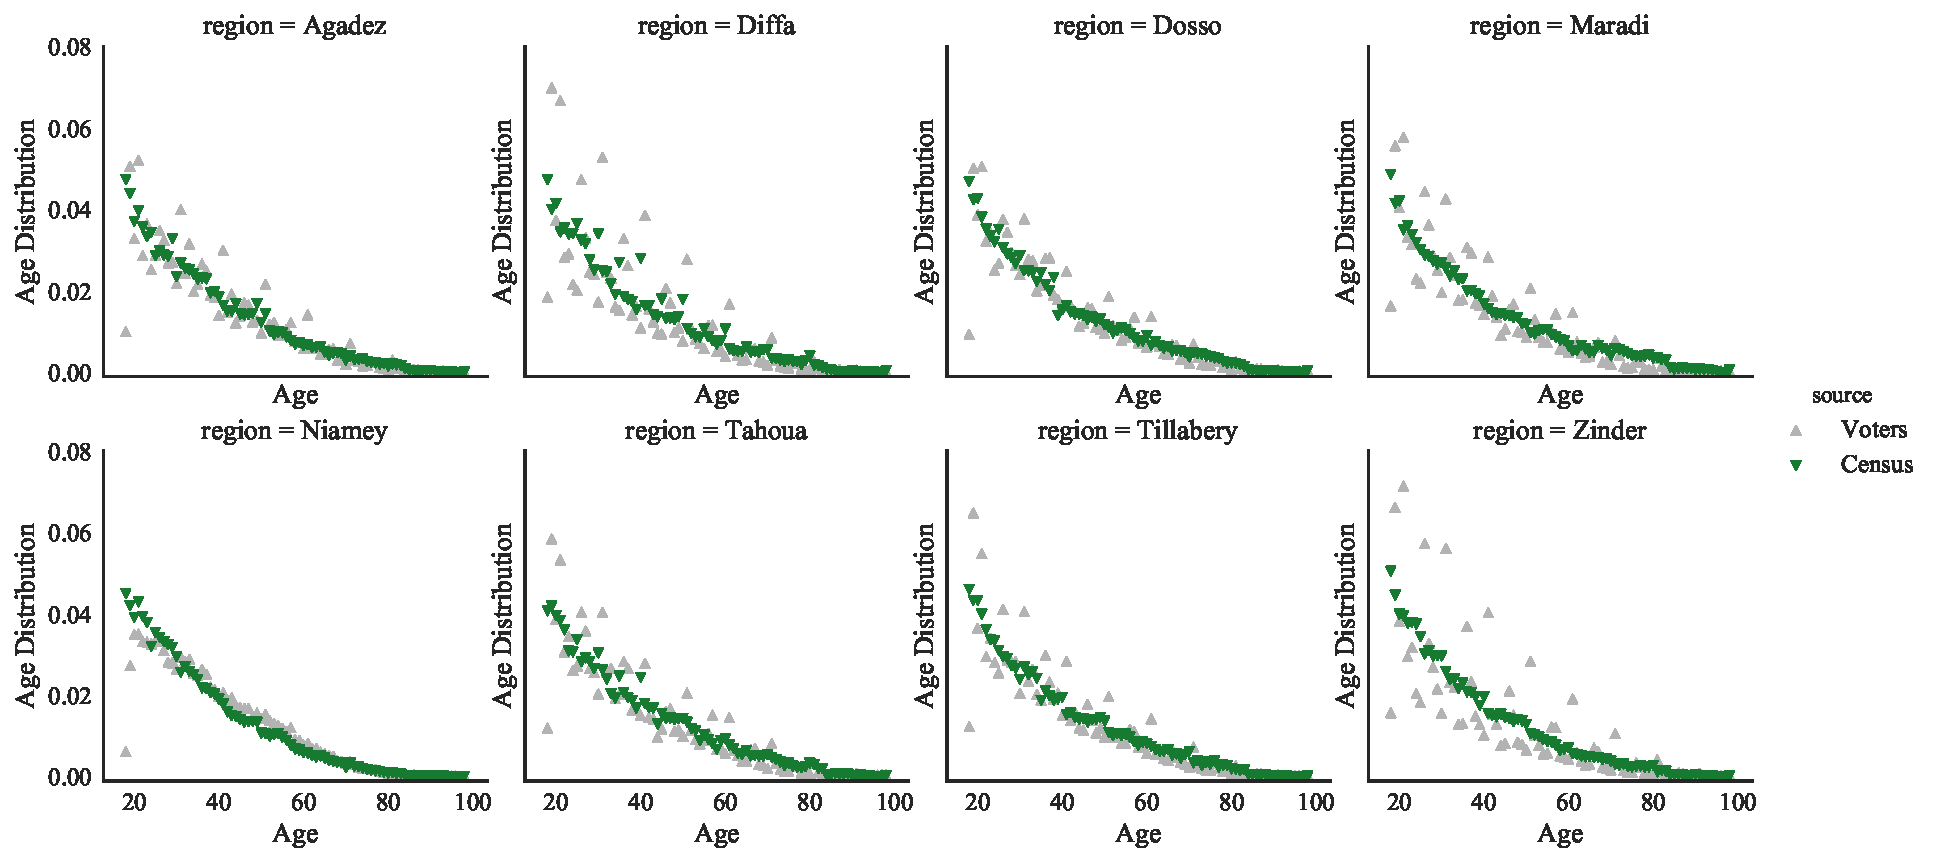
\includegraphics[width=\textwidth]{figure/age_structure_comparison.pdf}
		\caption{Comparison of standardized adult age distribution between the 2012 census and the 2016 voting lists}
		\label{fig:age_comparison}
	\end{center}
\end{figure}

A specificity of the voting list is that it does not include children under 18, as they are not allowed to vote. Additionally, the completeness of the data is not perfect, and I should assess and correct voters lists counts to correct this. Finally, as voting lists are very local, I will need to determine the most appropriate level of aggregation to get a meaningful estimation of the population age and gender distribution. Figure \ref{fig:age_comparison} compares the standardized age distribution of adults in the 2012 census and in the 2016 voters list at regional level. We can see there is more variability in the voters lists age structure than in the census. Concordance between the two age distributions seems to vary between regions.

We will model population size and age and gender distribution, using a life table method, using different life tables. Our gold standard will be the results from the 2012 census. We will compare performance of our approach applied at locality level, Health Zone level and regional level to choose the best performing approach.


\subsection{Output}

The output of the project for the quarter will  be to produce a dashboard, allowing display of our results for local practitioners. This dashboard will have the following feature :
\begin{enumerate}
	\item An interactive map of Niger localities, selectable by clicking, or panning for multiple selection
	\item An estimation of the population in the zone selected on the map
	\item A histogram representing the age structure of the population in the localities selected on the map
	\item A search box through which the user will be able to search for a given locality. Every name linked to a mapped locality will be searchable and will return the different matching localities in a hierarchized way.
\end{enumerate}



\subsubsection{Timeline}
\label{timeline:aim3}
I am currently trying to obtain more detailed census data from Niger Census. Meanwhile, the name matching and locality mapping work is already well advanced as we have a first set of matched names from the unsupervised approach, and I have already explored approaches to GPS correction for RENALOC. I anticipate three more months on the name matching and one month to confirm the locality mapping and the overlay with other \textit{adhoc} layers such as health services and health administration map, and should have completed mapping data by September 2017. I plan 5 months of work for the population estimation, and should have my final results by February 2018. Figure \ref{GanttPaper3} summaries this timeline.

\begin{figure}[t]
	\begin{ganttchart}[vgrid,hgrid,
	y unit chart=.6cm]{1}{18}
		\gantttitle{2017}{12}
		\gantttitle{2018}{6} \\
		\gantttitlelist{1,...,12}{1} \gantttitlelist{1,...,6}{1}\\

		\ganttset{bar/.append style={draw=green!40 , fill=green!40},
                    group/.append style={draw=green, fill=green}}
		\ganttbar{Data Extraction}{1}{3} \\
		\ganttbar{Name Matching}{1}{6} \\
		\ganttbar{Locality Mapping}{7}{9} \\
		\ganttmilestone{First complete map}{9} \\
		\ganttbar{Population Estimation}{10}{14} \\
		\ganttmilestone{Sharing Final Results}{14} \\
		\ganttbar{Paper Writing}{15}{16} \\
		\ganttbar{Dashboard Design}{15}{16} \\
		\ganttmilestone{Paper Submission}{16}
	\end{ganttchart}
	\caption{Gantt Chart for Aim 3}
	\label{GanttPaper3}
\end{figure}
